\section{Build}
Nachdem das Problem genauer analysiert und erste Ideen gesammelt und veranschaulicht wurden, wird nun nach dem ``Build - Measure - Learn'' Zyklus von Lean Startup \footnote{nach \citet{ries2014lean}} vorgegangen. Dieser Zyklus sollte dabei so iterativ wie möglich sein und am Ende jedes Zykluses sollten neue Insights bezüglich unseren aufgestellten Hypothesen vorliegen.

Im folgenden Kapitel wird der Aufbau der Entwicklungsumbegung sowie die Evaluierung der verschiedenen Technologien beschrieben. Anschliessend wird der Entwicklungsprozess genauer erläutert und erklärt wie der MVP getestet wird.

\subsection{Technologien}
Folgend werden die eingesetzten Technologien in der Arbeit erläutert. Dabei wird zuerst kurz auf die verwendete Backend Plattform eingegangen. Anschliessend den Cloudanbieter evaluiert und letztendlich auf das Framework für die Entwicklung der mobilen Applikationen eingegangen.

\subsubsection{Backend Technologie}
Als Backendlösung unserer Applikation haben wir uns für eine Serverless Lösung auch bekannt als ``FaaS'' (Function as a Service) und einige Dienste in Form von ``Software as a Service'' (SaaS) entschieden. Die bedeutet letztendlich, dass wir kein Webframework wie Java Spring oder Django als zentrales Backend verwenden, sondern unser Backend aus verschiedenen vorhandenen Services und Produkten zusammensetzen werden.

Der Entscheid in diese Richtung hatte folgende Hauptgründe: 
\begin{enumerate}
    \item Unser Backend ist nicht wirklich komplex, der Fokus liegt auf dem Frontend (komplexere Funktionen können für den MVP auch noch gemockt werden um an User Feedback zu kommen)
    \item Wir werden sehr viele Standardkomponenten verwenden wie eine Authentisierung oder das Speichern von Objekten mit CRUD Operationen. Ein eigenes Backend zu entwickeln und auf einen Server zu deployen wäre für die Entwicklung der Applikation ein Overhead gewesen.
    \item Die Applikation soll möglichst modular aufgebaut werden, sodass später auch eine eigene Backendlösung implementiert werden kann.
\end{enumerate}

\newpage
Konkret werden wir mindestens folgende Services brauchen:
\begin{enumerate}
    \item Authentifizierung
    \item Datenbank mit REST Interface
    \item Möglichkeit zur Ausführung von einfachen Funktionen
\end{enumerate}

\subsubsection{Cloud Anbieter}
Für Faas und SaaS gibt es aktuell zwei grosse Anbieter: AWS und Firebase. AWS ist der Service von Amazon und ist schon ein wenig älter. Es ist eine gute Gesamtlösung und sehr performant. Die einzelnen Services sind User friendly und der Support ist sehr gut\footnote{https://dashbird.io/blog/aws-lambda-vs-firebase/}. Zu den Nachteilen von AWS gehört, dass die Lernkurve relativ flach ist, wenn man bedenkt, dass es eine grosse Anzahl an Services gibt. Auch ist es eher auf grössere Projekte ausgerichtet und wenn man sich nicht gut auskennt, kann man schnell einmal mehr bezahlen, als man vorausberechnet hat.
Firebase ist ein etwas jüngerer Service von Google, der aber trotzdem sehr ausgereift ist und viele einzigartige Services anbietet. Es eignet sich eher für kleinere Projekte, da es einfach skalierbar ist und bis zu einer bestimmten Grenze gratis ist. Auf der anderen Seite kann es für grosse Datenmengen nicht mehr mit AWS mithalten und es gibt auch keine relationale Datenbank, was die Programmierung ein wenig schwieriger macht.
Wir haben uns schlussendlich aus folgenden Gründen für Firebase entschieden:
\begin{itemize}
    \item Gratis bis zu einer bestimmten Grenze. Danach ist eine monatliche Zahlung oder 'Pay as you go' möglich.
    \item Es werden viele nützliche Services angeboten, wie realtime Database, Authentication, Advertising, Analytics, A/B Testing, etc.
    \item Firebase wird von Google angeboten, weshalb es aktiv maintained wird und wahrscheinlich auch in Zukunft noch verfügbar sein wird.
    \item Firebase ist sehr einfach integrierbar in Android und iOS Apps, sowie auch in Web SDK's.
    \item Die Anwendung könnte nach Bedarf skaliert werden.
\end{itemize}

Bezogen auf die oben aufgeführten Services werden wir folgende Produkte von Firebase verwenden:
\begin{enumerate}
    \item Firebase Authentification\footnote{https://firebase.google.com/docs/auth}
    \item Firebase Cloud Firestore (Realtime NoSQL Datenbank mit REST Interface)\footnote{https://firebase.google.com/docs/firestore}
    \item Firebase Cloud Functions \footnote{https://firebase.google.com/docs/functions}
\end{enumerate}


\subsubsection{Mobile App Framework (Frontend)}
Da unsere App möglichst viele Smartphone Benutzer erreichen sollte, müssen wir eine Android und iOS Version erstellen. Das heisst, wir hätten für die Programmierung jeweils den doppelten Aufwand. Viel praktischer wäre es, eine einzige Codebase zu haben, mit der sich dann jeweils die Android und iOS App kompilieren lassen. Deshalb haben wir uns für das React Native Framework entschieden. Es bietet genau diese Funktionalität an und ist momentan Marktführend in diesem Bereich. Der wesentliche Unterschied von React Native gegenüber Konkurrenzprodukten liegt darin, dass React den Code in den jeweiligen Native Code umwandelt wodurch man fast keine Nachteile gegenüber Nativer App Entwicklung hat\footnote{https://www.polidea.com/blog/react-native-vs-native-app-developmentpros-and-cons-for-business/}. Andere Lösungen versuchen lediglich den Code und das UI wie ein Native App aussehen zu lassen, was oftmals in einer mühseligen Bastelei endet. Der einzige Nachteil gegenüber Nativer App Entwicklung ist, dass man nicht alle nativen Funktionalitäten verwenden kann. Bei iOS kann man bspw. das ARKit nicht verwenden. Eine einzige Codebase zu haben vereinfacht auch das Testing und Bugfixing.


\subsection{CI/CD}
Um einen MVP möglichst schnell an User verteilen zu können, muss  der Prozess des Buildens und Deployment automatisiert werden. Folgend werden unsere Überlegungen und Implementierungen einer CI/CD Pipeline dokumentiert. 

Da als Backend eine Kombination aus Firebase Services verwendet wird, ist eine CI/CD Pipeline nur für den Teil des Frontends notwendig.

\subsubsection{App Distribution}
Bevor wir uns weitere Gedanken über die automatisierte Auslieferung unserer Mobileapp machen können, muss zuerst definiert werden, über welche Plattform wir unsere App an die ersten User verteilen werden, um Feedback erhalten zu können. Beim Stichwort Mobile App Verteilung darf man natürlich die offiziellen App Stores von Apple und Google nicht unerwähnt lassen. Die offiziellen App Stores haben aber für Beta- bzw. Alphatests einige gravierende Nachteile:

\begin{enumerate}
    \item Apps werden besonders für den Apple App Store vor Release genau geprüft. Apps im Alpha oder Betastadium haben oft noch Fehler und Bugs. Solche Apps werden normalerweise nicht für den App Store zugelassen.
    \item Aufgrund der Prüfungen in den App Stores dauern Releases relativ lange. Auch Updates werden bei neuen Funktionalitäten geprüft und so kann ein Release schon einmal Tage dauern.
    \item Releast man eine Applikation bereits in sehr frühen Stadium in den offiziellen Stores so ist es für Nutzer bereits möglich die Applikation zu bewerten. Da man meist am Anfang noch mit Fehlern und Bugs rechnen muss, könnten sich so schlechte Reviews sammeln, welche anschliessend nicht mehr so einfach verbessert bzw. angepasst werden können.
\end{enumerate}

Aus diesem Grund gibt es nebst der klassischen App Stores diverse Plattformen und Apps von Erst- und Drittanbietern, welche speziell für das schnelle Testen von Mobile Apps konzipiert wurden. Folgend werden drei mögliche Plattformen miteinander verglichen und dabei Vor- und Nachteile aufgelistet.

\textbf{Apple TestFlight}

Mit TestFlight hat Apple eine eigene Plattform für Alpha- und Betatests im Angebot. Tester müssen sich die TestFlight Applikation im AppStore herunterladen. Mithilfe eines Einladungsmail oder eines Opt-in Links können sich interessierte Tester als Betatester registrieren und können sich die Applikation anschliessend auf das iOS Gerät herunterladen.

\underline{Vorteile:} Bis zu 10'000 Tester möglich, Direktes Feedback in der Testflightapp möglich

\underline{Nachteile:} Nur auf iOS verfügbar, Apple prüft die Applikation trotzdem, jedoch weniger streng

\textbf{Google Play Beta}

Im Google Play Store ist es im Gegensatz zu iOS möglich direkt Alpha- oder Betatests durchführen zu können. Der Entwickler kann dabei zwischen ``Closed Beta'', wo Nutzer mithilfe eines Google Accounts eingeladen werden müssen oder einer offenen Beta, welche auch im Play Store angezeigt wird, wählen.

\underline{Vorteile:} Nutzer müssen keine zusätzliche Applikation herunterladen. Offene Betas können im Play Store entdeckt werden.

\underline{Nachteile:} Nur für Android verfügbar, Review durch Google

\textbf{HockeyApp / Visual Studio App Center}

Früher unter dem Namen ``HockeyApp'' bekannt bietet auch Microsoft eine Plattform fürs schnelle Testen von Applikationen an. Auch hier muss eine Applikation auf das Gerät installiert werden, um an der Beta teilnehmen zu können. Mit dem App Center bietet Microsoft zudem eine komplette Plattform für CI/CD, Analytics, Push Notifications und weiteres an.

\underline{Vorteile:} iOS und Android können mit einer Plattform abgedeckt werden. Gute Integration in die App Center Plattform mit vielen anderen Funktionen

\underline{Nachteile:} Es muss eine zusätzliche Applikation installiert werden.

Letztendlich haben wir uns für die Lösung mit dem Visual Studio App Center entschieden. Besonders der Vorteil, sämtliche Distribution über dieselbe Platform lösen zu können hat uns zu diesem Entscheid geführt. Ausserdem sind weniger Prüfstellen involviert, was schlussendlich zu schnelleren Deployments führt.

\subsubsection{CI/CD Pipeline für Mobile App}
Nachdem klar war, wie die App beim Nutzer landet, musste nun noch evaluiert werden, wie der ganze Build und Release Prozess automatisiert werden konnte. 

CI/CD Lösungen gibt es relativ viele. Hier wurden auch wieder drei Lösungen in Betracht gezogen und miteinander verglichen.

\textbf{Jenkins}

Jenkins gehört zu den ``Urgesteinen'' der CI/CD Tools. Obwohl es bereits einige Jahr alt ist, wird es im Business Umfeld immer noch häufig genutzt. 

\underline{Vorteile:} Grosse Community und viel Know-How, Ausgereifte Software mit vielen Plugins, sehr flexibel

\underline{Nachteile:} Muss sehr viel selbst erstellt werden, keine offizielle Cloud Lösung (es gibt jedoch viele verschiedene Cloudplattformen von Drittanbietern für Jenkins)

\textbf{Gitlab CI/CD}

Das Git Repo Gitlab hat seit 2016 einie eigene Lösung für CI/CD. Gitlab CI/CD läuft nach Wahl auf eigener Infrastruktur oder direkt auf der Plattform von Gitlab. 

\underline{Vorteile:} Hosting direkt bei Gitlab möglich, sehr flexibel

\underline{Nachteile:} Integration mit VS App Center als Distributor schwierig

\textbf{Visual Studio App Center} 

Mit dem App Center hat Microsoft nebst der oben erwähnten App Distribution Plattform auch gleich eine eigene Plattform für CI/CD im Angebot. Diese ist speziell für Mobile Apps optimiert und hat alle Voreinstellung für React Native bereits konfiguriert.

\underline{Vorteile:} All-in-One Plattform für Mobile Apps, kann sich mit jedem Git Repo verbinden, Perfekte Integration mit Distribution

\underline{Nachteile:} Nur für Mobile App geeignet (wenig Flexibilität)

Letztendlich haben wir uns auch hier für das App Center entschieden, da es mit Abstand die schnellste und einfachste Lösung im Zusammenhang mit der Distribution ist. Folgend wird der Aufbau der Pipeline genauer erläutert.

\textbf{Aufbau der Pipeline}

Abbildung \ref{fig:cicd_pipeline} zeigt der Aufbau unserer Pipeline. Die beiden Tools die für die Pipeline verwendet werden ist Gitlab als Git Repository und VS App Center als CI/CD Tool.
Wir werden unsere Applikation aufgrund des sogennante Gitlows\footnote{https://www.atlassian.com/git/tutorials/comparing-workflows/gitflow-workflow} implementieren. Dabei wird für jedes Feature ein eigener Branch erstellt, welcher vom ``Develop'' Branch abgespalten wird. Ist ein Feature fertig, wird ein Pull-Request nach Develop erstellt und von den anderen gereviewt. Ist alles in Ordnung wird der Branch nach Develop gemergt und die erste CI/CD Pipeline wird gestartet. 

Nachdem Gitlab die App Center Pipeline getriggert hat, werden Unittests und ein JS Linting ausgeführt. Anschliessend wird hier nur die Android App gebuildet und an die Entwickler gesendet. Es wird für den Test nur Android verwendet, da alle Mitglieder des Teams nur Android Telefone haben. Die Mitglieder bekommen ein E-Mail und können nun die Applikation testen. Integrationstests werden aufgrund des relativ grossen Aufwands nicht automatisiert ausgeführt (siehe Kapitel \ref{testing} Testing).

Ist der Test erfolgreich verlaufen, so kann nun ein Pull Request auf den Master Branch eröffnet werden. Wird dieser gemergt so werden nun die Release Pipelines getriggert. Auch hier werden nocheinmal die Tests und Linting ausgeführt, anschliessend werden die Apps für iOS und Android gebuildet und an die Alphatester gesendet. Diese können die Applikation nun sofort herunterladen und erhalten nach Wunsch eine Push Benachrichtigung, wenn ein neuer Release verfügbar ist.

\begin{figure}[H]
    \centering
    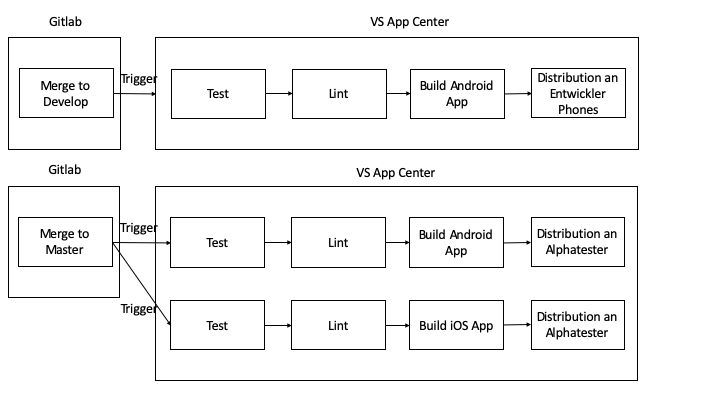
\includegraphics[width=\textwidth]{images/CICD.png}
    \caption{Diagramm CI/CD Pipeline}
    \label{fig:cicd_pipeline}
\end{figure}

Diese Konzeption der Pipeline ist bereits so implementiert. Abbildung \ref{fig:cicd_overview} zeigt ein Screenshot der Weboberfläche des VS App Centers.

\begin{figure}[H]
    \centering
    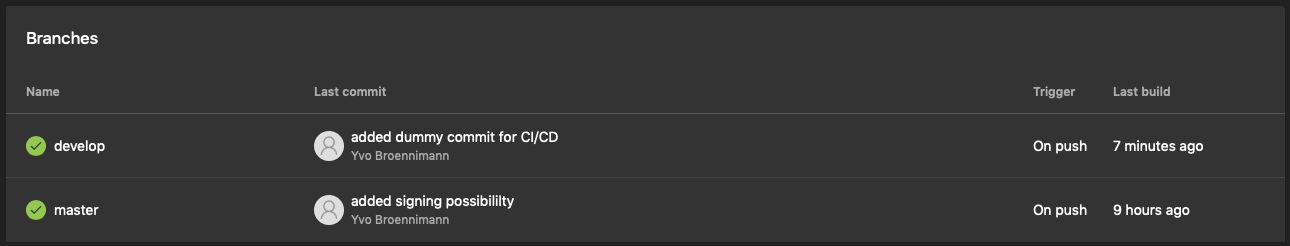
\includegraphics[width=\textwidth]{images/Overview_CICD.png}
    \caption{Screenshot der beiden Build Pipelines}
    \label{fig:cicd_overview}
\end{figure}

Der aktuelle Stand unserer Applikation kann unter dem untenstehenden Link heruntergeladen werden. Aktuell unterstützt die Version nur Android ist jedoch bereits vollständig automatisiert. Der Build für iOS wird noch nachgereicht, da wir dort noch auf das Zertifikat warten müssen:

\href{https://install.appcenter.ms/users/yvo.broennimann/apps/the-gamechanger/distribution_groups/alphatesters}{Download Link Android}


\subsection{Testing} \label{testing}
Continous Integration bzw. Continous Delivery wären ohne automatisierte Tests nicht wirklich sinnvoll. Folgend wird kurz auf die möglichen und verwendeten Testframeworks eingegangen.

\textbf{Unittests}

Für React-Native gibt es relativ viele verschiedene Testing Frameworks. Wir haben uns für das offiziell von Facebook empfohlene Testing Frame ``Jest'' entschieden. Mithilfe von Jest lassen sich einerseits Funktionen wie klassisch bei Unittests testen. Darüber hinaus bietet Jest jedoch die Möglichkeit des Snapshot Testings an: Mithilfe des Snapshot Testings lassen sich Komponenten der React-Native Applikation sehr schnell und einfach auf korrektes Rendering überprüfen. Dabei werden den einzelnen Komponenten bestimmte Properties und Stateinformationen übergeben und die gerenderte View welche aus den Properties resultiert wird als JSON gespeichert. Wird dieses View nun unbewusst geändert und hat somit einen anderen Wert als sie beim Erstellen des Snapshots hatte, so schlägt der Test fehl. Somit kann sehr schnell getestet werden, ob die Komponenten alle richtig rendern. Die Funktionalität der Komponenten muss natürlich manuell mit Unittests getestet werden.

\textbf{Integrationtests}

Integrationtests bzw. End2End Tests sind für React-Native deutlich komplexer. Das Problem ist, dass für den Test ein iOS bzw. Android Simulator gestartet werden muss. Automatisiert auf VS App Center können diese Simulatoren nicht ausgeführt werden. Lokale Frameworks für das End2End Testing wären bspw. Detox\footnote{https://github.com/wix/Detox} oder Apium\footnote{https://github.com/appium/appium}. Bei beiden Frameworks können gewisse Schritte definiert werden, wie bspw. ``Click auf Navigationstab 3'' und anschliessend das erwartete Output definiert werden. Bei der Ausführung wird der Simulator gestartet und überprüft, ob der vorher definierte Output mit dem Output auf dem Simulator übereinstimmt. Beide diese Frameworks sind jedoch sehr aufwändig zu implementieren. Für dieses Projekt werden wir die Applikation jeweils vor dem Release von Hand testen. 

VS App Center hat jedoch zusätzlich noch ein Feature namens ``Test on real devices'', welches sehr einfach in die Release Pipeline integriert werden kann. Mithilfe dieses Features lassen sich zwar keine Tests definieren, jedoch wird die Applikation auf verschiedenen echten Geräten wie Google Pixel oder Samsung Galaxy S10 gestartet und es werden zufällige Eingaben gemacht. Started die Applikation auf allen Geräten und stürzt nicht ab so sind diese Tests bestanden. Wir werden dieses Feature in späteren Versionen noch einbauen, da dies nur mit dem Premium Plan von VS Code Center verfügbar ist und die Tesversion nur 30 Tage dauert. Das Feature kann jedoch mit einem Klick in der Pipeline aktiviert werden.

\subsection{Beispiel einer OpenAPI Definition}

Da wir als Backend eine Kombination aus SaaS und FaaS verwenden, haben wir nur den Teil der Userverwaltung und Login als Beispiel einer OpenAPI Definition konzipiert.
Abbildung \ref{fig:openapi_methods} zeigt dabei die erstellten Endpoints. Es wurden Endpoints für Login, Logout, Abfrage für alle User mit bestimmten Filterkriterien sowie Abfrage 
eines spezifischen Users anhand der ID erstellt.

\begin{figure}[H]
    \centering
    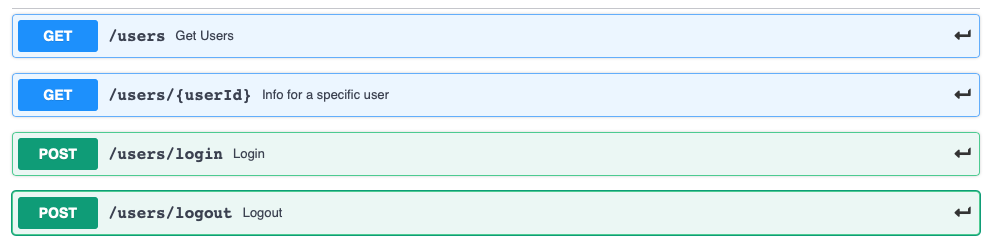
\includegraphics[width=\textwidth]{images/swagger_overview.png}
    \caption{Screenshot der OpenAPI Methoden}
    \label{fig:openapi_methods}
\end{figure}

Bei der Abfrage nach User können noch die zwei Filter- oder Suchparameter ``Region'' und ``Name'' als URL Parameter mitgegeben werden.

\begin{figure}[H]
    \centering
    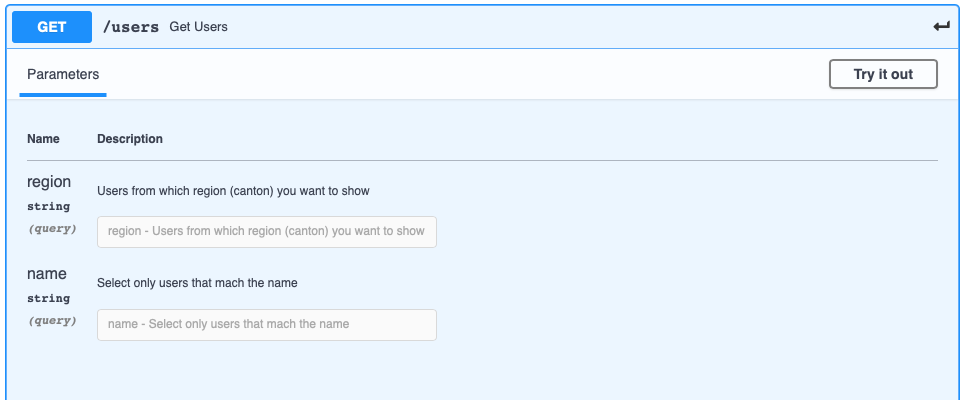
\includegraphics[width=\textwidth]{images/swagger_get_users.png}
    \caption{Beispiel GET Users}
    \label{fig:openapi_get_users}
\end{figure}

Abbildung \ref{fig:openapi_code} zeigt noch den Code zur in Abbildung \ref{fig:openapi_get_users} dargestellten Funktion.
Mithilfe von Swagger lassen sich sehr schnell API Definitionen erstellen. Besonders gut gefallen hat uns, dass man sogenannte
Schemas erstellen kann, in welchen man verschiedene Objekte wie etwas ``User'' oder ``Tiere'' definieren kann. Möchte man anschliessend
die als JSON serialisierte Version zurückgeben, so kann einfach nur noch auf das Schema referenziert werden. Die richtige Serialisierung
macht Swagger anschliessend automatisch.

Desweiteren ist es sehr beeindruckend, dass man sich anhand der OpenAPI Definition für praktisch jedes einigermassen verbreitete Webframework
Code generieren lassen kann. Da man in Swagger auch oft vergessene Dinge wie korrektes Errorhandling einfach definieren kann, spart man so
sehr viel Zeit, da dies auch automatisch im Code abgebildet wird. Im Grunde genommen braucht man nun nur noch die Datenbankanbindung und die Business
Logic zu implementieren. Das ganze mühsame Bootstrapping der API übernimmt Swagger. Zudem gibt es auch praktische Codegeneration Features fürs Frontend,
wo die API Endpoints bereits praktisch in Methoden verpackt sind, welche einfach aufgerufen werden können.

Wie sich zeigt ist also Swagger respektive OpenAPI deutlich mehr als nur eine Schnittstellenbeschreibung oder API-Dokumentation. Es kann
besonders am Anfang der Entwicklung sehr gut dabei helfen sich auf das wesentliche der API zu konzentrieren und nimmt mühsames Bootstrapping durch die
Codegeneration ab. Der Wert der Dokumentation darf jedoch nicht unterschätzt werden: Besonders wer sich schon durch mehrere Tausend Zeilen Source Code
quälen musste, um den richtigen Endpoint mit der richtigen Parametrisierung zu kommen, wünscht sich überall eine solch genaue Dokumentation mit OpenAPI.
Einzige Bedingung ist dann aber natürlich auch das Nachführen der Definitionen.

\begin{figure}[H]
    \centering
    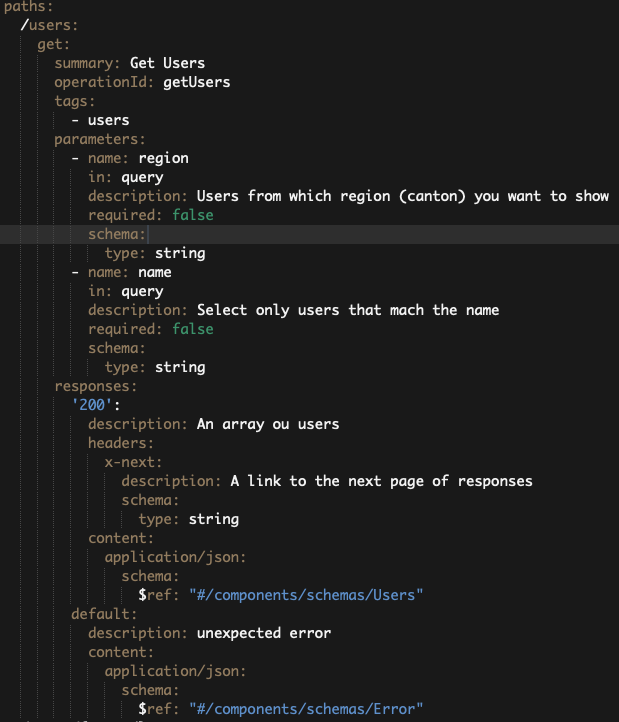
\includegraphics[width=0.8\textwidth]{images/swagger_code.png}
    \caption{Code zu GET Users}
    \label{fig:openapi_code}
\end{figure}

\subsection{Authentifizierung mit Firebase Auth und Datenmodell im Firestore}
Beim Betätigen des \say{Sign in with Google}-Buttons wird der User über OAuth mit Hilfe seiner Google Account Credentials authentifiziert. Danach erhält der User ein JWT Token, mit welchem die Applikation die Firebase Firestore API anspricht um Userspezifische Daten anzufordern. Dieser gesamte Autentisierungsprozess ist mit Firebase Authentication direkt in unserem Firebase Projekt integriert, sodass wir spezifisch für dieses Projekt eine Userverwaltung haben. Dies erlaubt es uns auch über die Firebase Konsole einzelne User zu sperren oder die Anzahl neuer Anmeldungen einzusehen. 
\newpage
\begin{figure}[h]
    \centering
    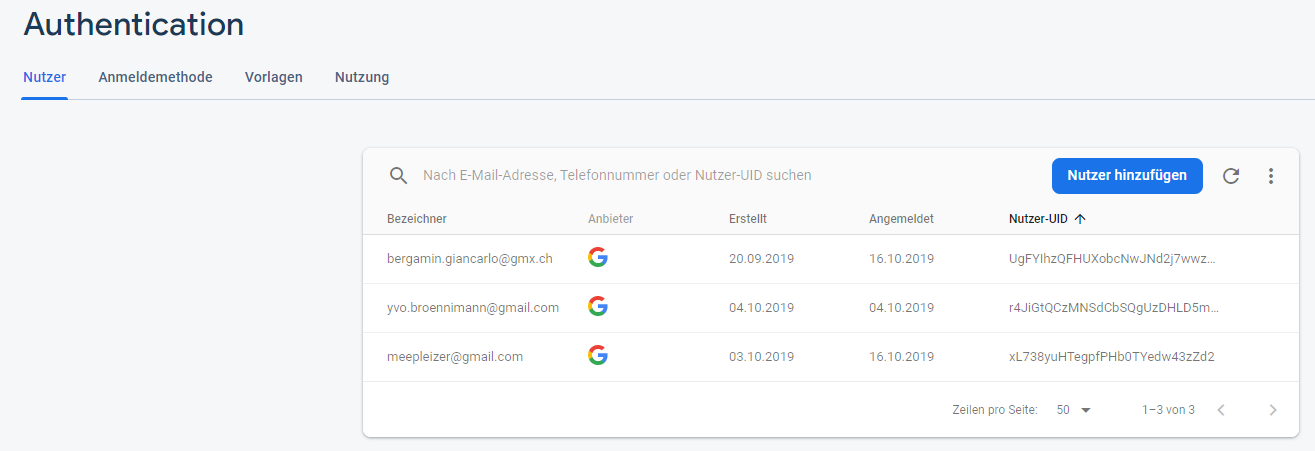
\includegraphics[width=\textwidth]{images/firebaseauth.PNG}
    \caption{Userverwaltung}
    \label{fig:userverwaltung}
\end{figure}

Der zweite Service von Firebase, welchen wir gebrauchen ist der Firestore. Der Firestore ist eine NoSQL Datenbank, welche aus zwei Komponenten besteht: \textbf{\textit{Documents und Collections}}. \textbf{Documents} sind Dokumente, in welchen Key-Value Paare gespeichert werden. \textbf{Collections} sind Sammlungen von Documents. Im Unteren Beispiel gibt es also eine Sammlung \say{users}, welche zwei Documents enthalten. Ein Userdocument beinhaltet Userdaten wie zum Beispiel der Name des Users, das Alter des Users und das Beitrittsdatum des Users (in der Abbildung ganz rechts). Das Userdocument enthält aber auch eine Subcollection namens future\_sessions, welche wieder eine Collection darstellt, in der zukünftige Brettspielsessions in eigenen Documents zusammengefasst sind. 

\begin{figure}[h]
    \centering
    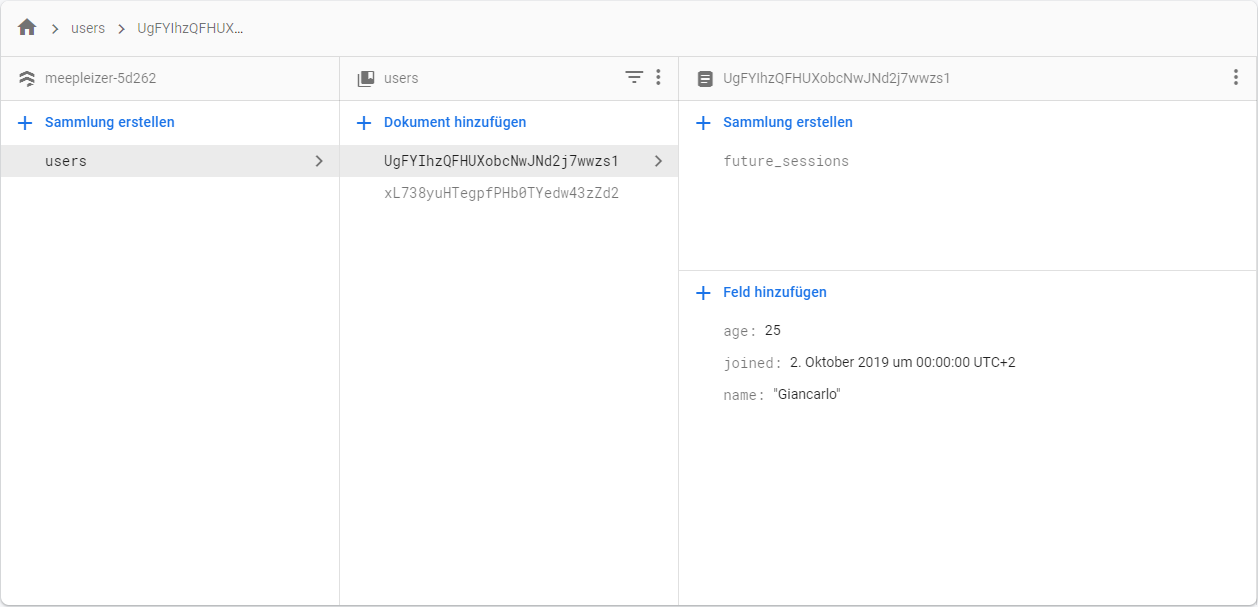
\includegraphics[width=\textwidth]{images/firestore_document.PNG}
    \caption{Firestore Document und Collection}
    \label{fig:document_collection}
\end{figure}

Das Datenmodell des Firestores ist also hierarchisch aufgebaut und wechselt ab zwischen Collections und Documents wie schematisch in der unteren Abbildung dargestellt.

\begin{figure}[h]
    \centering
    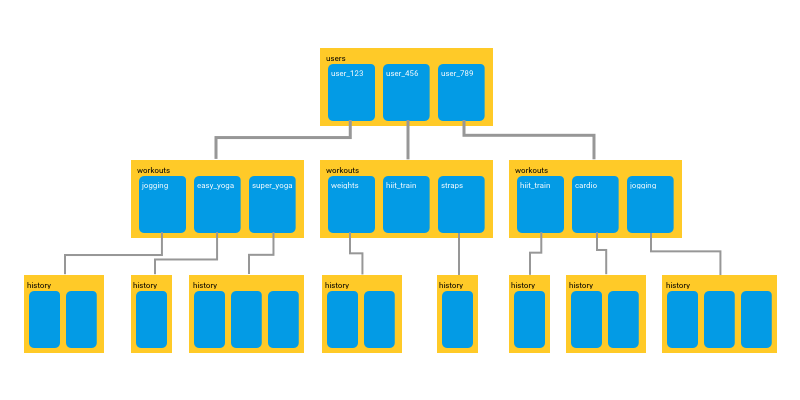
\includegraphics[width=\textwidth]{images/firestore.png}
    \caption{Datenmodell Firestore}
    \label{fig:firestore}
\end{figure}


Das JWT Token, welches wir über den Authentisierungsprozess erhalten haben, können wir jetzt nutzen, um Userspezifische Daten anzufordern. Die Autorisierung des User wird mit sogenannten Security Rules direkt in der Firebase Firestore Database erledigt. Eine solche Security Rule sieht so aus:

\begin{figure}[H]
    \centering
    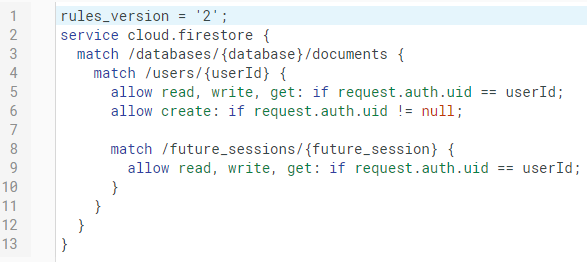
\includegraphics[width=\textwidth]{images/security_rule.PNG}
    \caption{Security Rule Firestore}
    \label{fig:security_rule}
\end{figure}


Diese Regel besagt zum Beispiel, dass ein User mit einer seiner UserID auf sein User Dokument in der Collection \say{Users} zugreifen kann (Zeile 4 in der Abbildung oben). Diese Security Rules vererben die Rechte nicht an Subcollections, deshalb müssen wir dem User auch den spezifischen Zugriff auf seine \say{future\_sessions} geben (Zeile 8 in der Abbildung oben).
\newline
Das dargelegte Beispiel repräsentiert das Datenmodell der ersten beiden Komponenten des Authentisierungs Screens und des Haupt Screen, wobei beim Haupt Screen zu diesem Zeitpunkt erst die zukünftigen Sessions angezeigt werden und noch keine erhaltenen Einladungen oder abgeschlossene Sessions. Diese Funktionalität müssen wir in einem weiteren Inkrement entwicklen. 


\subsection{Sicherheit}
Folgend wird auf die verschiedenen Aspekte bezüglich Security im Frontend und Backend des Projekt eingegangen.

\subsubsection{Bestimmung des Schutzbedarfs}
Um den Schutzbedarf der Daten von The Gamechanger zu bestimmen, wurde die Einstufungstabelle der Schutzbedarfsanalyse des Informatik Steuerorgans des Bundes\footnote{Zu finden unter: \url{https://www.isb.admin.ch/isb/de/home/ikt-vorgaben/prozesse-methoden/p041-schutzbedarfsanalyse_schuban.html}} ausgefüllt. Das Resultat wird in Abbildung \ref{fig:einstufung_schutzbedarf} gezeigt. 

\begin{figure}[H]
    \centering
    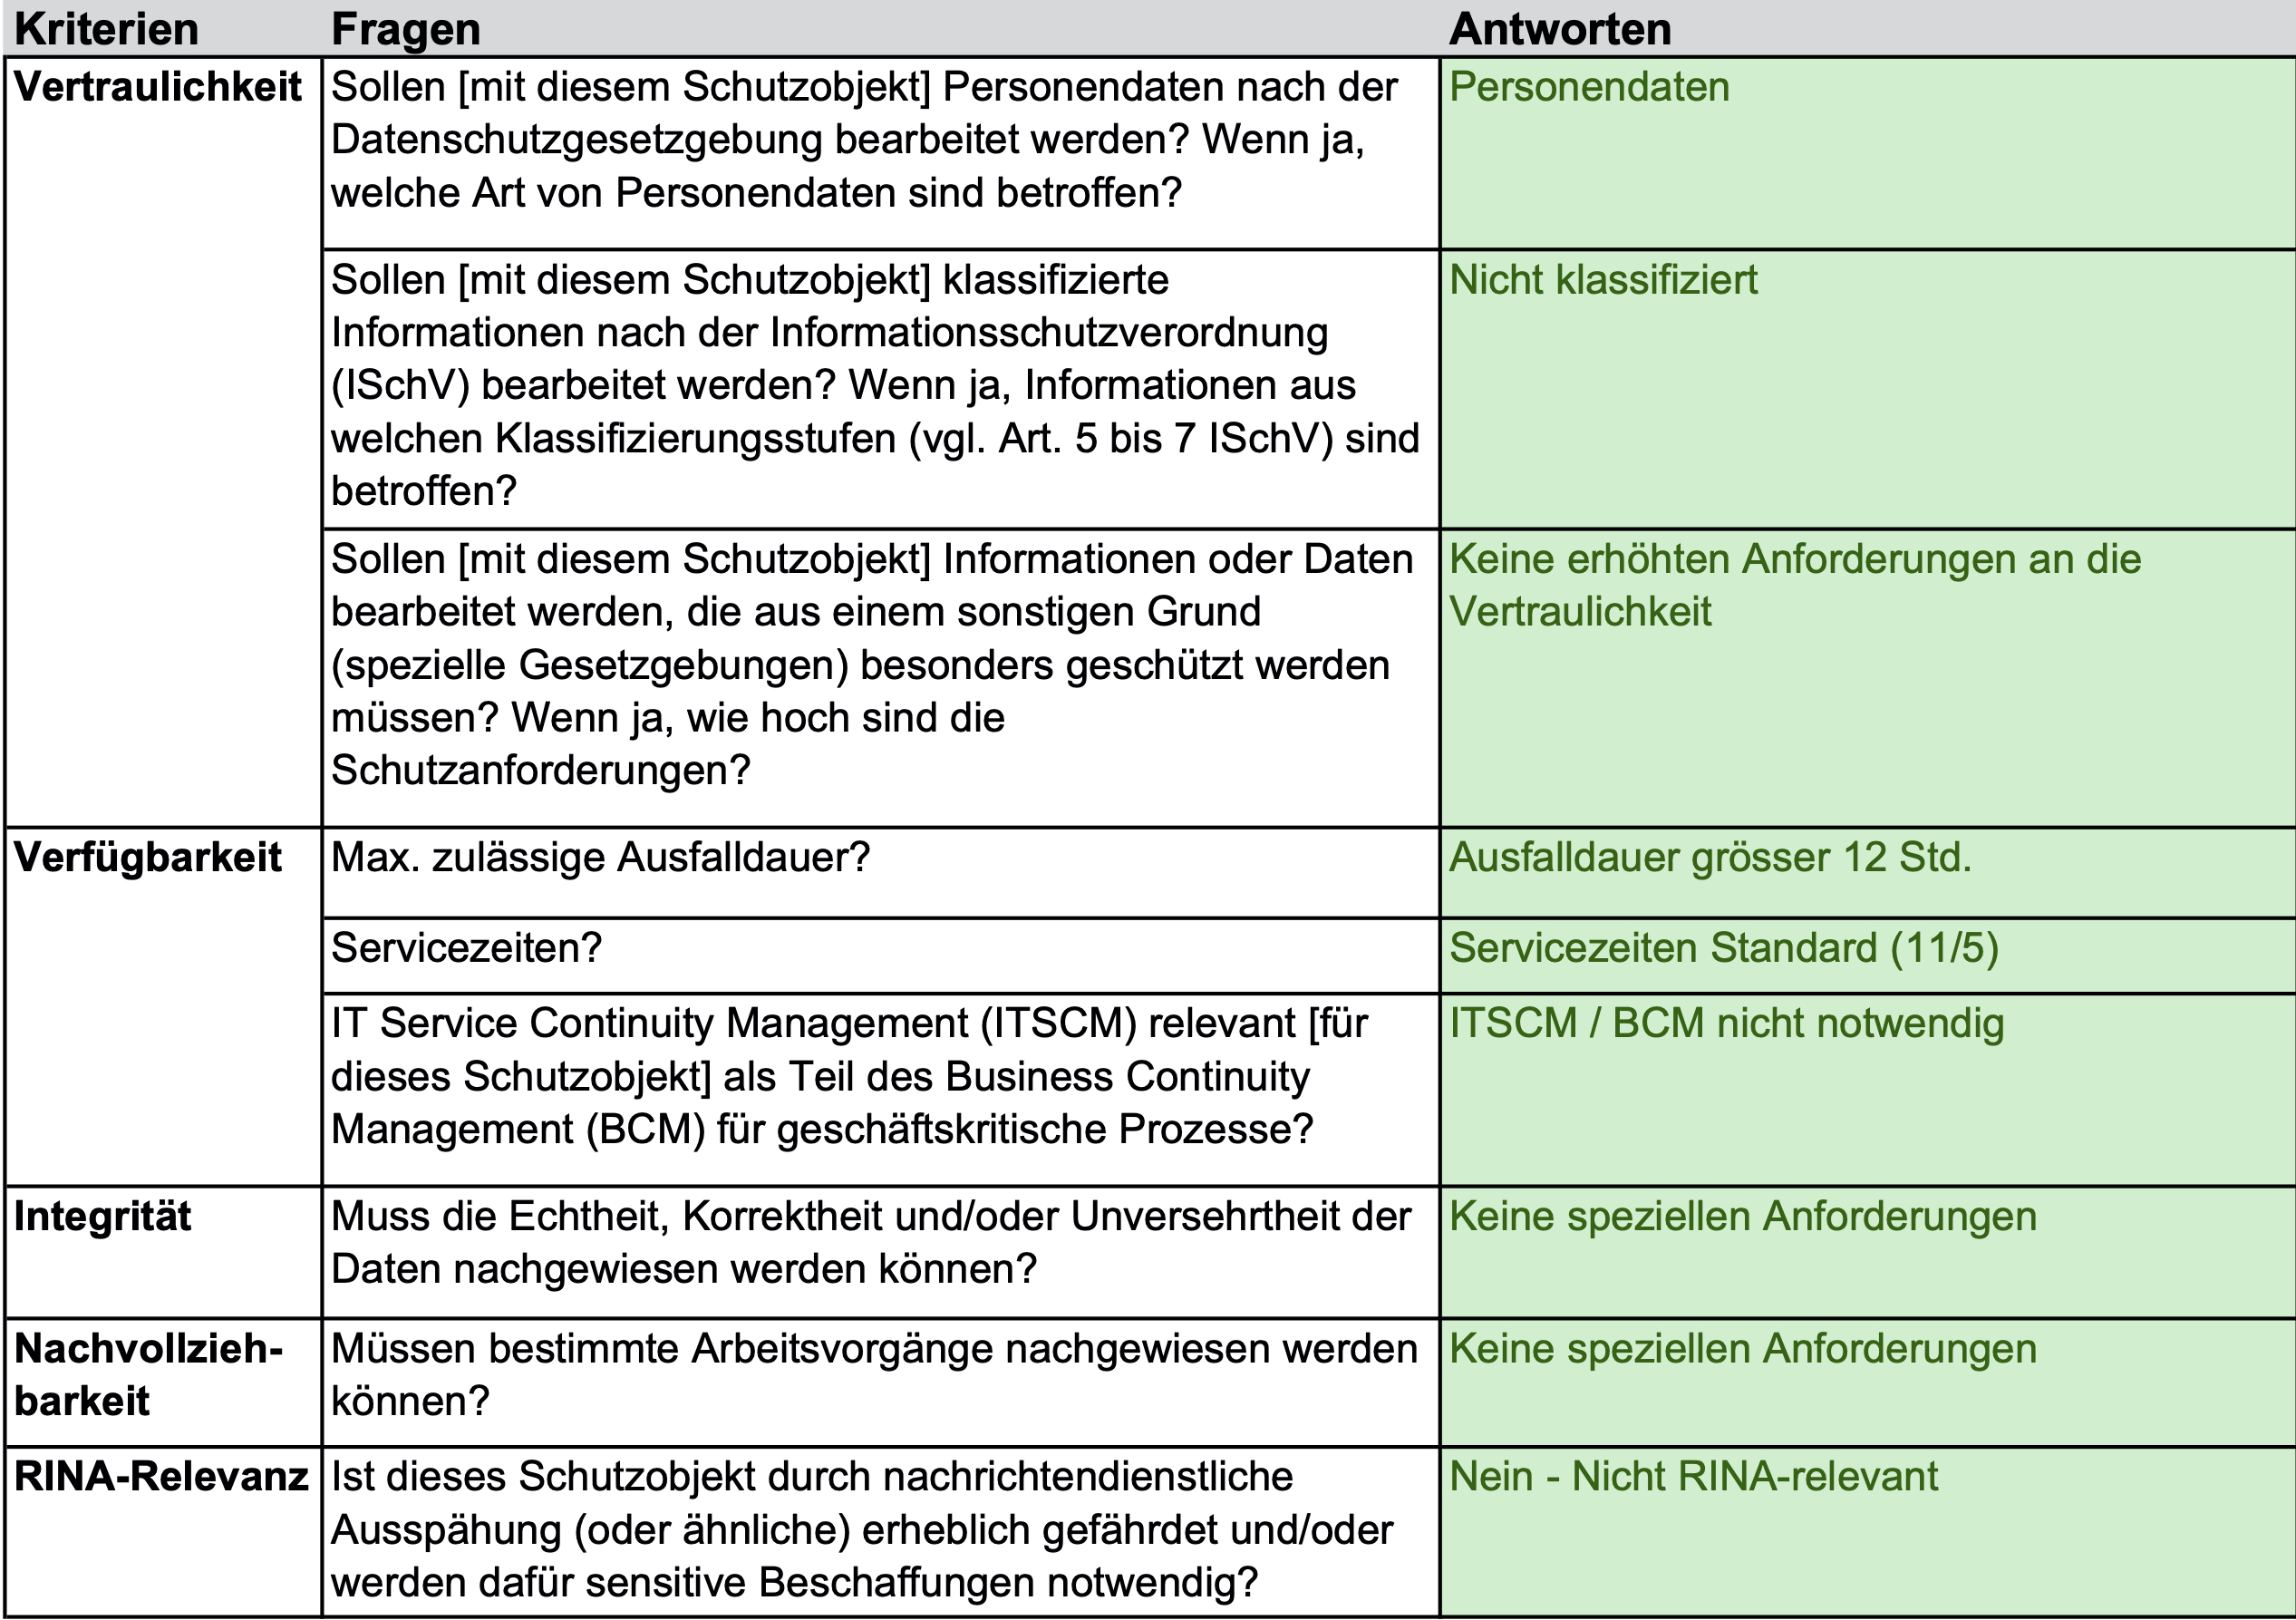
\includegraphics[width=\textwidth]{images/Einstufung_Schutzbedarf.jpg}
    \caption{Einstufung Schutzbedarf}
    \label{fig:einstufung_schutzbedarf}
\end{figure}

Die einzigen Daten, die The Gamechanger von den Benutzern verwendet, sind der Name und eine E-Mail Adresse. Dies sind Personendaten, die jedoch keine erhöhten Anforderungen an die Vertraulichkeit stellen. Bezüglich der Verfügbarkeit der Daten bestehen auch keine erhöhten Anforderungen. Wenn die App mal ein Tag offline sein sollte, würde man evtl. einige E-Mails von Benutzern erhalten, jedoch würde dadurch direkt kein relevanter Geldverlust zustande kommen (höchstens weniger Werbeeinnahmen, falls Werbung aufgeschalten werden sollte). Die Anforderungen an die Nachvollziehbarkeit sind auch im normalen Rahmen und die Daten sind auch nicht durch nachritendienstliche Ausspähung (oder ähnliches) gefährdet. 

\subsubsection{NPM Vulnerability Audit}
Da wir die mobile Applikation mit Hilfe des React Native Frameworks machen, sammeln sich schnell sehr viele Abhängigkeiten in Form von 3rd party NPM Packages an. Zum jetzigen Zeitpunkt beinhalted der \say{node\_modules} Ordner, welche alle Dependencies files beinhaltet, schon 684 Unterordner. Man kann sich vorstellen, dass diese Anzahl an Dependencies manuell nicht mehr überprüfbar ist und man keine manuellen Sicherheitschecks mehr durchführen kann. NPM biete daher eine Funktion namens \say{npm audit}, welche diese Dependencies automatisch auf Vulnerabilities überprüft. Das haben wir dann auch gemacht und unten ist der Audit Report abgebildet.


\begin{figure}[H]
    \centering
    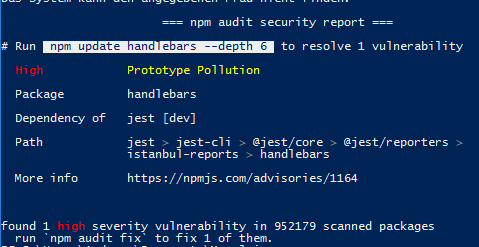
\includegraphics[width=\textwidth]{images/npm_audit.PNG}
    \caption{NPM Audit Security report}
    \label{fig:security_report}
\end{figure}

Man sieht, dass eine Vulnerability gefunden wurde und diese als \say{High}
eingestuft wurde. Man sieht auch in welchem Modul diese Vulnerability besteht und über einen Link bekommt man dann sogar noch mehr Informationen über die gefundene Schwachstelle. Die unten abgebildete Darstellung zeigt diese ausführliche Information. Dabei wird die Schwachstelle beschrieben und es wird aufgezeigt, was ein Angreifer machen könnte, falls diese Schwachstelle ausgenutzt werden würde. In unserem Fall könnte ein Angreifer durch die Schwachstelle bösartigen Code ausführen (Remote Code Execution). Man sieht auch, wann diese Vulnerability gemeldet wurde. In diesem Fall wurde die Schwachstelle am 16. September 2019 gemeldet, sie ist also relativ neu.


\begin{figure}[H]
    \centering
    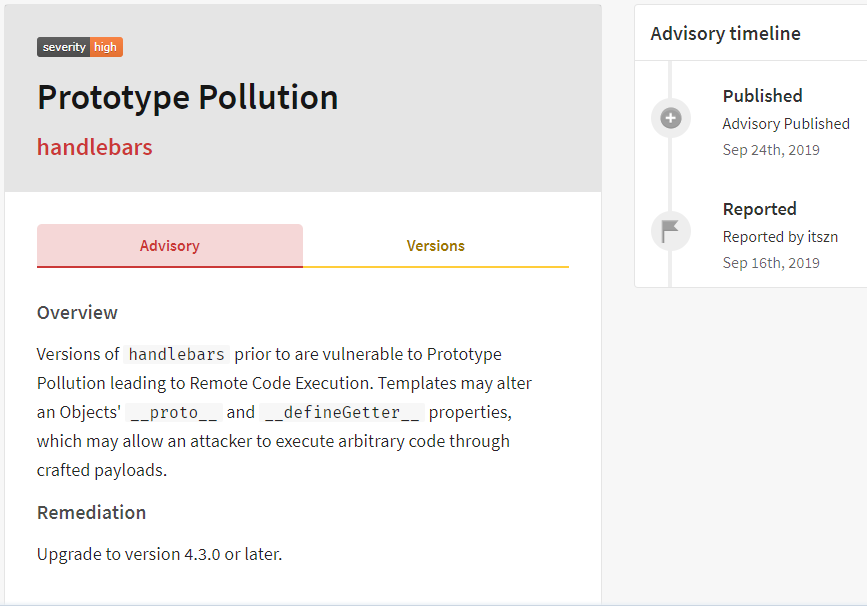
\includegraphics[width=\textwidth]{images/vulnerability_info.PNG}
    \caption{Weitere Informationen über die Schwachstelle}
    \label{fig:vulnerability_information}
\end{figure}

Zum Glück bietet NPM auch gerade die dazu passende Funktion, um die gefundenen Schwachstellen zu mitigieren, indem die betroffenen Module auf eine Version aktualisiert werden, in der die Schwachstelle geschlossen ist.

\begin{figure}[H]
    \centering
    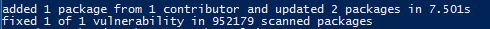
\includegraphics[width=\textwidth]{images/fixed_vulnerability.PNG}
    \caption{Output von npm audit fix}
    \label{fig:vulnerability_fixed}
\end{figure}

Damit wurde das betroffene Modul aktualisiert und die Schwachstelle geschlossen.
\newline
Es ist natürlich wichtig, dass man dieses Audit regelmässig durchführt, da natürlich immer wieder neue Schwachstellen entdeckt werden und man diese so schnell wie möglich schliessen sollte. Es würde sich also auch anbieten, dieses Audit in der CI/CD pipeline einzubinden, um bei Änderungen der Appliaktion auch automatisch ein Audit durchzuführen.


\subsubsection{OWASP Mobile Top Ten}
Das OWASP Mobile Security Project hat 2016 eine Liste mit den Top 10 Mobile Vuilnerabilities herausgegeben, welche kreiert worden ist, um das Sicherheitsbewusstsein der Entwickler zu fördern und um auf die gravierendsten Sicherheitsthemen in der Mobile Entwicklung aufmerksam zu machen. In diesem Abschnitt schauen wir uns kurz zwei Themen dieser OWASP Mobile Top 10 an und versuchen dabei unsere Applikation in diesen Kontext zu stellen.

\paragraph{M3 Insecure Communication}
Die Beschreibung dieser Vulnerability lautet wie folgt: \textit{\say{This risk covers all aspects of getting data from point A to point B, but doing it insecurely. It encompasses mobile-to-mobile communications, app-to-server communications, or mobile-to-something-else communications. This risk includes all communications technologies that a mobile device might use: TCP IP, WiFi, Bluetooth Bluetooth-LE, NFC, audio, infrared, GSM, 3G, SMS, etc.}}\footnote{https://www.owasp.org/index.php/Mobile\_Top\_10\_2016\-M3\-Insecure\_Communication}

Die Kommunikation mit anderen Services ist bei unserer Applikation zentral. Deshalb sehen wir in dieser unsicheren Kommunikation eines der grössten Risiken. Ein Beispielszenario lautet wie folgt: \textit{\say{\textbf{Privacy information leakage}: The mobile app transmits personally identifiable information to an endpoint via non-secure channels instead of over SSL. This jeopardizes the confidentiality of any privacy-related data between the mobile app and the endpoint.}}

Es ist deshalb sehr wichtig, dass die gesamte Kommunikation zu Google Firebase verschlüsselt statt findet. Dies stellen wir sicher, indem wir die von Google bereitgestellten Client-Side Libraries verwenden, um mit dem Online Service zu kommunizieren. Auch die Authentikation wir mit Hilfe von Google Libraries durchgeführt. Dadurch dass wir diese, von Spezialisten entwickelten Libraries verwenden und diese Funktionalität nicht selber implementieren, können wir zu einem grossen Teil Implementationsfehler vermeiden.

\paragraph{M7 Poor Code Quality}
Auch diese Sicherheitsthema ist für uns relevant. Die Beschreibung lautet auch hier wie folgt:
\textit{\say{This is the catch-all for code-level implementation problems in the mobile client. That's distinct from server-side coding mistakes. This captures the risks that come from vulnerabilities like buffer overflows, format string vulnerabilities, and various other code-level mistakes where the solution is to rewrite some code that's running on the mobile device.}}

Es geht also um programmiersprachspezifische Funktionen, welche bei unvorsichtiger Programmierung dazu führen können, das Sicherheitsprobleme auftreten. Ein typisch Beispiel dafür wäre der berühmte Buffer Overflow in C Sprachen. Da wir mit JavaScript arbeiten (und indirekt auch mit Java und Swift) und da sprachspezifische Methoden verwenden, welche den Buffer Overflow nicht möglich machen, sind wir da zum Teil gut abgesichert. Natürlich existiert immer die Gefahr unsichere Methoden zu verwenden, insbesondere dann, wenn man 3rd-party Libraries verwendet und die Implementation dieser Funktionen nicht kennt. 
Eine Möglichkeit dieses Risiko zu minimieren, ist es so zu programmieren, dass der Source Code gut lesbar und verständlich ist und man auch eine ausführliche Dokumentation des Codes erstellt. 
Memoryleaks können allgein zu Problemen führen und man sollte die Applikation gut auf solche Probleme überprüfen.






\subsubsection{Bestimmung der Massnahmen}
Nach der Schutzbedarf mithilfe des Excels bestimmt wurde, wurde nun auch das Excel für die konkreten Massnahmen für den Grundschutz durchgearbeitet. Folgend werden die wichtigsten Punkte daraus zusammengefasst und die konkrete Implementierung erläutert:

\textbf{Kryptografie}
\begin{itemize}
    \item Kryptografische Verfahren müssen dem Stand der Technik entsprechen
    \item Zertifikate können nicht von Schweizer CA ausgestellt werden, aber anerkannter CA ist vorhanden
	\item Kryptografische Schlüssel müssen sicher Verwaltet und
	\item gespeichert werden. In unserem Fall ist das Konkret das Zertifikat, um mit Firebase zu kommunizieren, sowie die Zertifikate um die Android und iOS App zu signieren. Diese werden verschlüsselt abgespeichert (In unserem Falle befinden sich diese in 1Password. Eine skalierbare Lösung wäre bspw. HashiCorp Vault\footnote{https://www.vaultproject.io}. Hier können solche Daten und Passwörter zentral und sicher abgespeichert werden.
\end{itemize}

\textbf{Betriebssicherheit}
\begin{itemize}
    \item Schutz vor Malware: Die gesamte IKT muss durch aktuell gehaltene Software vor Schadsoftware Befall geschützt werden. Folgende Stellen können potentielle Orte für Malware sein:
    \begin{itemize}
        \item  NPM Packages können unsichere Teile aufweisen, welche ermöglichen könnten, dass Daten abgezogen oder verändert werden
        \item Auf Android wäre es auch möglich, dass Malware auf den Geräten installiert ist, welche die Daten der Applikation klauen könnten. Bei iOS ist es weniger problematisch, da dort die Richtlinien zur Installation von Software deutlich höher sind.
    \end{itemize}
    \item Aufzeichnung und Überwachung: Folgende Aktivitäten sind (möglichst in pseudonymer Form) für IKT-Systeme und Anwendungen zweckgebunden und nachvollziehbar aufzuzeichnen, zu überwachen und zeitnah auszuwerten:
    \begin{itemize}
        \item Gescheiterte Authentifikationsversuche (inklusive eindeutiger Identifikation der Herkunft)
        \item Gescheiterte Objektzugriffe
        \item  Vergabe und Änderung von Privilegien
        \item  Alle Aktionen, die erhöhte Privilegien benötigen.
    \end{itemize}
    \item  Schwachstellenmanagement: Ist vor allem für NPM Packages wichtig. Diese müssen regelmässig überprüft werden.
    \item OWASP Top Ten: Hier macht es vor allem sind die Mobile OWASP Top Ten zu betrachten\footnote{https://www.owasp.org/index.php/OWASP\_Mobile\_Top\_10}. Diese konzentrieren sich auf die speziellen Sicherheitsanforderungen von Mobile Apps.
\end{itemize}

\textbf{Kommunikationssicherheit}
\begin{itemize}
    \item  Verschlüsselung mit TLS: Sämtliches Datenverkehr muss verschlüsselt über HTTPS laufen.
\end{itemize}

\subsubsection{Statische Codeanalyse bezüglich Security}
Eine Massnahme welche zwar keine manuellen Security Reviews oder Penetrationstests ersetzt, sind statische Codeanalysen. Hierbei wird der Source Code auf mögliche Sicherheitslücken analysiert. Statisch bedeutet in diesem Falle, dass der Code nie ausgeführt wird sondern einfach auf bestimmte Patterns im Code geachtet wird, welche eine Sicherheitsbedrohung darstellen könnten.

Bevor wir ein System zur statischen Codeanalyse implementiert haben, wurde eine kurze Evaluierung der aktuell beliebtesten Produkte durchgeführt. Das aktuell bekannteste und verbreitetste Programm zur statischen Codeanalyse bezüglich Security ist ``Checkmarx''. Checkmarx läuft auf einem Server und kann sehr simpel in eine CI/CD Pipeline integriert werden, da es Scanner für relativ viele unterschiedliche Programmiersprachen zur Verfügung stellt. Checkmarx ist jedoch nur kommerziell erhältlich und relativ teuer, weshalb es für dieses Projekt nicht in Frage kam. Eine Alternative, welche zwar nicht ganz so mächtig bezüglich Security Analyse aber dafür kostenlos ist, stellt die Software ``SonarQube'' dar. SonarQube ist eigentlich nicht umbedingt direkt für Security Checks konzipiert worden, jedoch wurde es im Laufe der Zeit mit immer mehr Security Checks erweitert. Da es das einzige Tool ist, dass wir gefunden haben, welches komplett kostenlos ist, haben wird uns für dieses entschieden.

\textbf{Implementierung}

SonarQube ist praktischerweise als Docker Container erhältlich und kann als erster Test sehr simpel lokal ausgeführt werden. Auf dem Hostsystem muss nur die SonnarScanner Software installiert werden und ein simples Konfigurationsfile erstellt werden. Mithilfe der Scanner Software kann anschliessend das ganze React Native Projekt automatisiert und schnell einerseits auf Sicherheitslücken andererseits auch gleichzeitig auf unschöne Codestellen, sogenannte ``CodeSmells'' überprüft werden. Abbildung \ref{fig:sonar_overview} zeigt die Übersicht der Analyse. 

\begin{figure}[H]
    \centering
    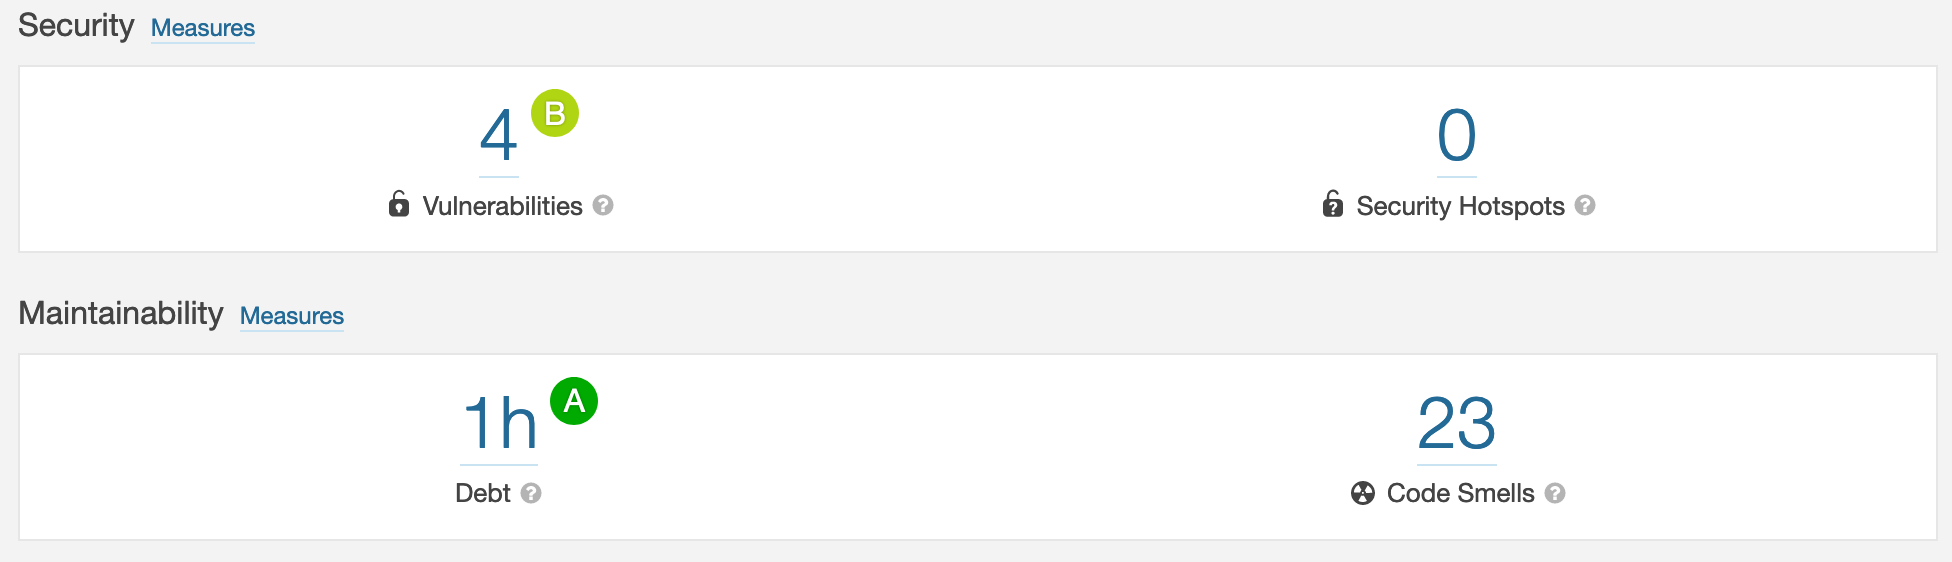
\includegraphics[width=\textwidth]{images/sonar_overview.png}
    \label{fig:sonar_overview}
    \caption{Übersicht Analyse SonarQube}
\end{figure}

Nebst einiger CodeSmells konnten 4 Minor Vulnerarbilities gefunden werden. Die genauere Analyse zeigte anschliessend, dass es sich bei den Vulnerabilities um Alerts handelt, welche zurzeit noch zu Debugging Zwecken im Code sind. (siehe Abbildung \ref{fig:sonar_security}). SonarQube begründet die Warnung wie folgt: ``alert(...) as well as confirm(...) and prompt(...) can be useful for debugging during development, but in production mode this kind of pop-up could expose sensitive information to attackers, and should never be displayed.''.

Unserer Meinung nach ist Sonar hier etwas ``übervorsichtig'', jedoch verstehen wir natürlich, dass dies bei einer produktiven Applikation eine Anlaufstelle für Hacker sein kann.

\begin{figure}[H]
    \centering
    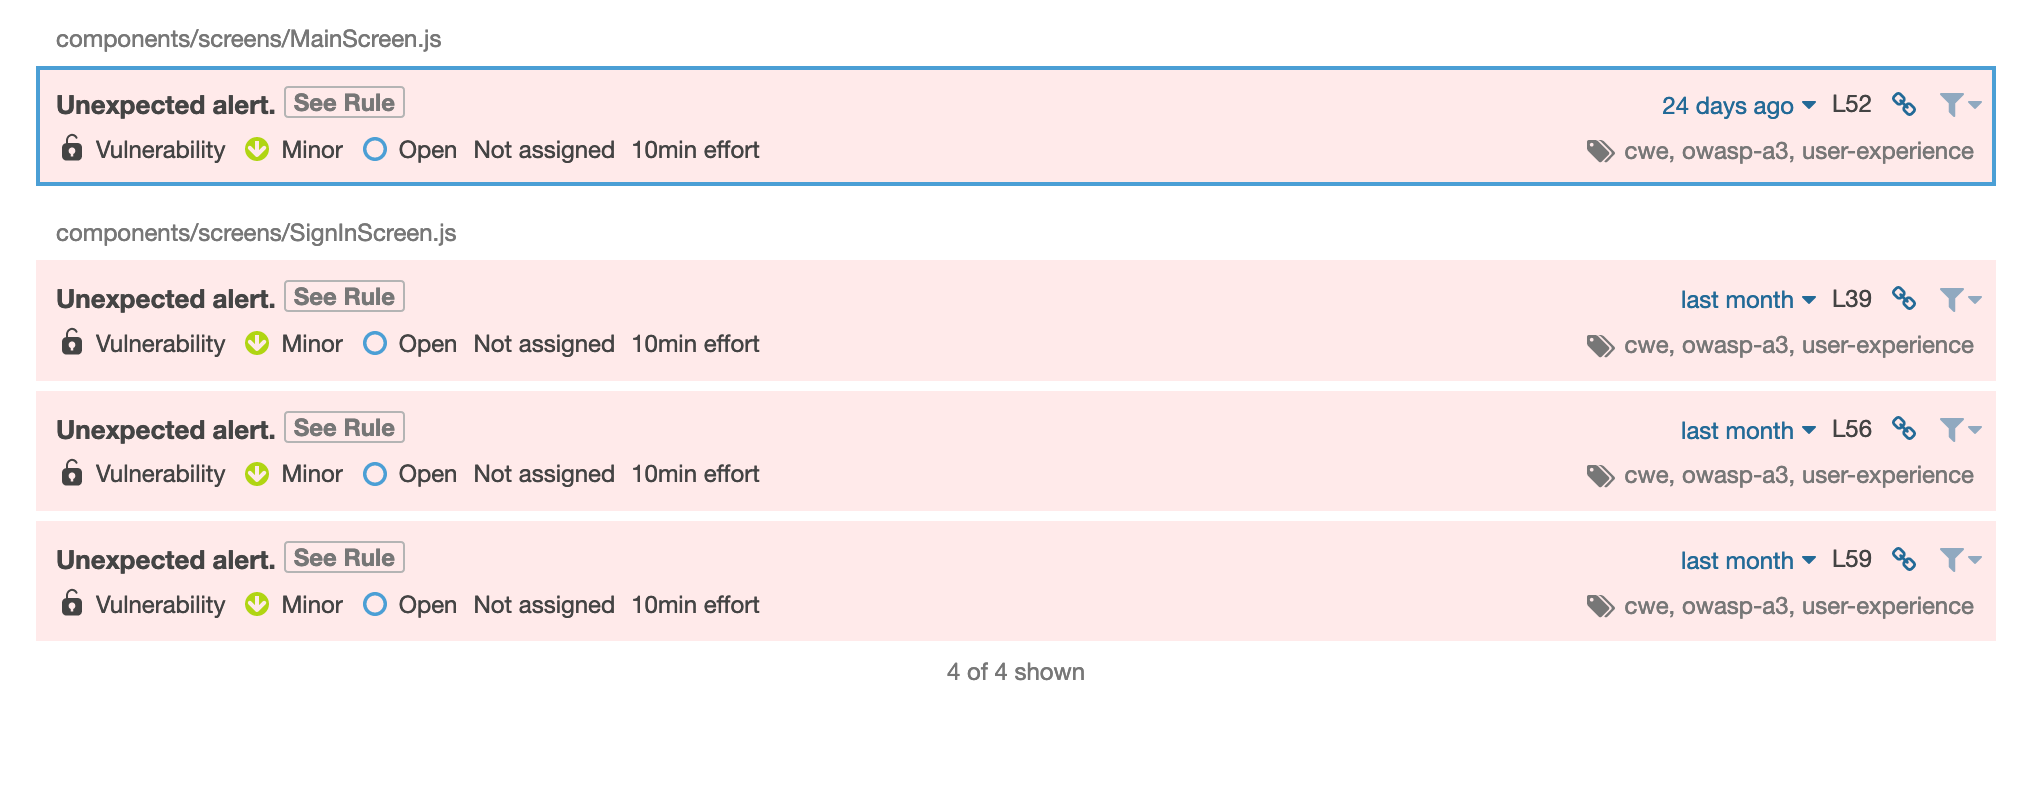
\includegraphics[width=\textwidth]{images/sonar_details.png}
    \caption{Security Probleme SonarQube}
    \label{fig:sonar_security}
\end{figure}

\subsubsection{Security seitens Firebase}
Bisher wurde vor allem auf das Frontend des Projekts eingegangen. Beim Backend haben wir mit Firebase nur relativ wenige Möglichkeiten was die Implementierung von Security angeht. Dies kann einerseits als Vorteil angesehen werden, da man sich relativ sicher sein kann, dass Google bei der Grösser und Verbreitung von Firebase gut Sicherheitsmechanismen eingebaut hat, jedoch ist man letztendlich Google relativ ausgeliefert. Hätte man nun sehr schützenswerte Daten wie Persönlichkeitsprofile so müsste man sich überlegen, ob man dieses Vertrauen einer Drittperson abgeben kann. Eine Möglichkeit um diesen Faktor zu beseitigen oder zumindest abzuschwächen wäre die vollständige Verschlüsselung der Daten auf Clientseite. Anschliessend würden nur die verschlüsselten Daten auf Firebase gespeichert.

Da wir es bei unseren Daten wie erläutert nicht um heikle Personendaten handelt werden wir die Daten nicht verschlüsselt bei Firebase speichern. Folgend fassen wir kurz die ``Privacy und Security Agreements'' von Firebase zusammen:

Firebase ist komplett GDPR compliant. Bei der Erklärung was das nun konkret bedeutet verweist Google auf den Link zu den Vorlagen des GDPR \footnote{https://eur-lex.europa.eu/legal-content/EN/TXT/?uri=CELEX\%3A32016R06}. Desweiteren hat Firebase diverse Security ISO Normen wie ISO 27001, ISO 27017, ISO 27018 und ist Privacy Shield Compliant nach EU und Schweizer Richtlinien. Sämtliche Kommunikation, extern als auch intern, ist mit TLS 1.2 verschlüsselt. Einiger Wehrmutstropfen gibt es aber schon: Firebase wertet sehr viele Daten der End User wie Crash Traces, IP Adressen, Passwörter und E-Mail Adressen aus. Offiziell wird dies als notwendig für die korrekte Funktiosweise des Services angegeben, jedoch muss man natürlich auch in Betracht ziehen, dass zwar die Plattform praktisch kostenlos ist, Google jedoch trotzdem irgendwie etwas verdienen muss. Hier ist es einfach nicht direkt Geld sondern Daten. Desweitern kann im Gegensatz zu anderen Cloudplattformen wie AWS oder Azure nicht ausgewählt werden, in welchem Land die Daten gespeichert werden sollen.\footnote{Quelle: https://firebase.google.com/support/privacy}